\documentclass[tikz,border=12pt]{standalone}
\usepackage[utf8]{inputenc}
\usepackage[T1]{fontenc}
\usepackage{lmodern}
\usepackage{array}
\usepackage{tikz}
\usetikzlibrary{arrows.meta,calc}
\definecolor{greenFill}{HTML}{E8F5E9}
\definecolor{greenStroke}{HTML}{43A047}
\definecolor{coreFill}{HTML}{E1F5FE}
\definecolor{coreStroke}{HTML}{0277BD}
\newcommand{\classcontent}[2]{\begin{tabular}{p{5.8cm}}\centering\bfseries #1\tabularnewline\hline\raggedright\arraybackslash #2\end{tabular}}
\begin{document}
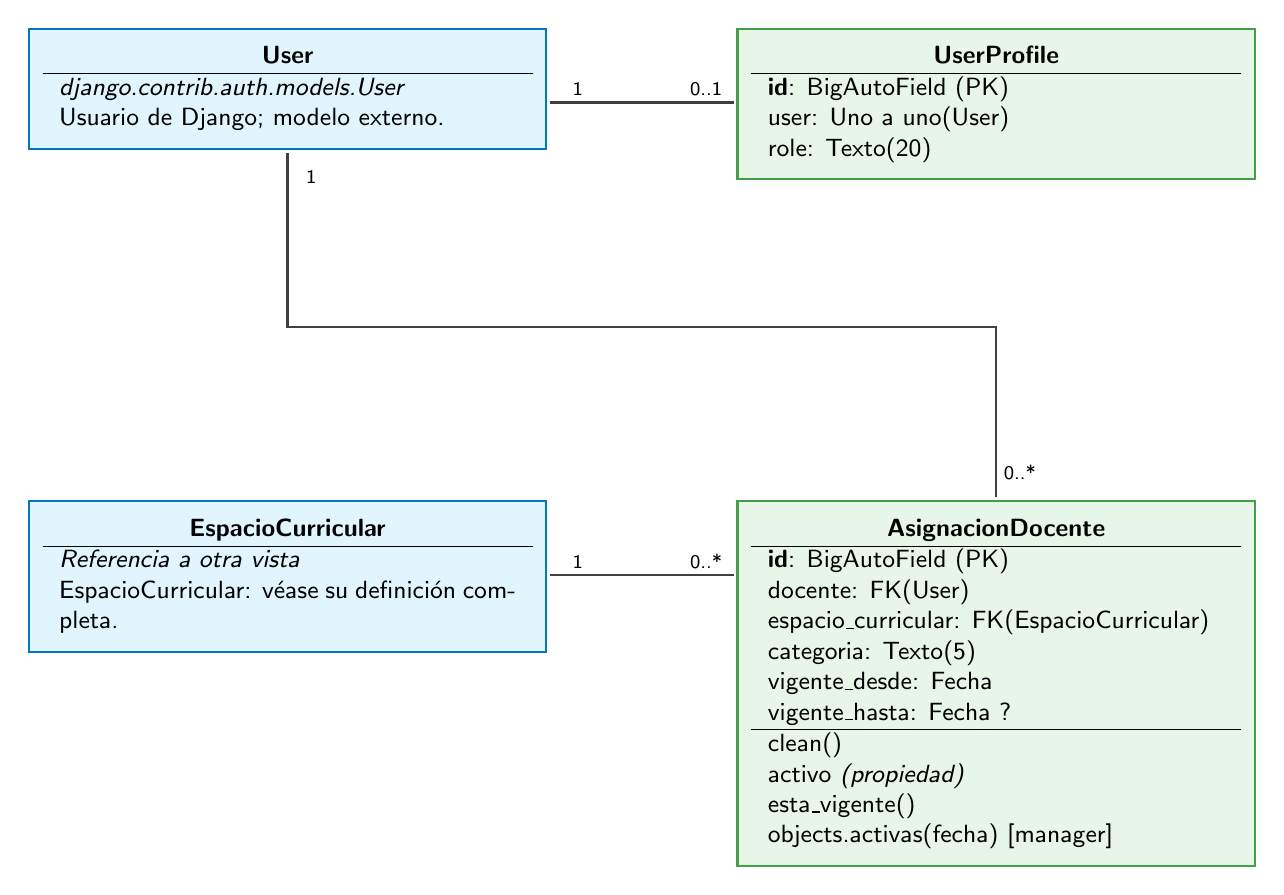
\begin{tikzpicture}[
 font=\sffamily\small,
 cls/.style={rectangle,draw=greenStroke,fill=greenFill,line width=.8pt,inner sep=5pt,anchor=north},
 ref/.style={cls,draw=coreStroke,fill=coreFill},
 association/.style={line width=.9pt,draw=black!75,shorten >=1pt,shorten <=1pt},
 dependency/.style={association,dashed,-{Stealth[length=3mm,width=2.2mm]}},
 mult/.style={font=\sffamily\scriptsize,fill=white,inner sep=2pt,text=black}
]
\node[ref] (User) at (0,0) {\classcontent{User}{\textit{django.contrib.auth.models.User}\\Usuario de Django; modelo externo.}};
\node[cls] (UserProfile) at (9,0) {\classcontent{UserProfile}{\textbf{id}: BigAutoField (PK)\\user: Uno a uno(User)\\role: Texto(20)}};
\node[ref] (EspacioCurricular) at (0,-6) {\classcontent{EspacioCurricular}{\textit{Referencia a otra vista}\\EspacioCurricular: véase su definición completa.}};
\node[cls] (AsignacionDocente) at (9,-6) {\classcontent{AsignacionDocente}{\textbf{id}: BigAutoField (PK)\\docente: FK(User)\\espacio\_curricular: FK(EspacioCurricular)\\categoria: Texto(5)\\vigente\_desde: Fecha\\vigente\_hasta: Fecha ?\\\hline clean()\\activo \textit{(propiedad)}\\esta\_vigente()\\objects.activas(fecha) [manager]}};
\draw[association] ($(User.north east)+(0,-.95)$) -- ($(UserProfile.north west)+(0,-.95)$) node[pos=.16,above,mult]{1} node[pos=.84,above,mult]{0..1};
\draw[association] ($(EspacioCurricular.north east)+(0,-.95)$) -- ($(AsignacionDocente.north west)+(0,-.95)$) node[pos=.16,above,mult]{1} node[pos=.84,above,mult]{0..*};
\draw[association] (User.south) -- (0,-3.8) -- (9,-3.8) -- (AsignacionDocente.north);
\node[mult] at ($(User.south)+(.3,-.35)$) {1};
\node[mult] at ($(AsignacionDocente.north)+(.3,.35)$) {0..*};
\end{tikzpicture}
\end{document}
